\section{視覚と行動の end-to-end 学習により経路追従行動をオンラ
インで模倣する手法}
1 章でも述べたが,本研究室の岡田ら\cite{okada2020}はメトリックマップベースの経路追従行動を end-to-end 学習を用いて模倣学習することで,視覚に基づくナビゲーション手法を提案した.
岡田らが提案するシステムを\figref{fig:okada_sys}に示す.

\begin{figure}[htbp]
  \centering
   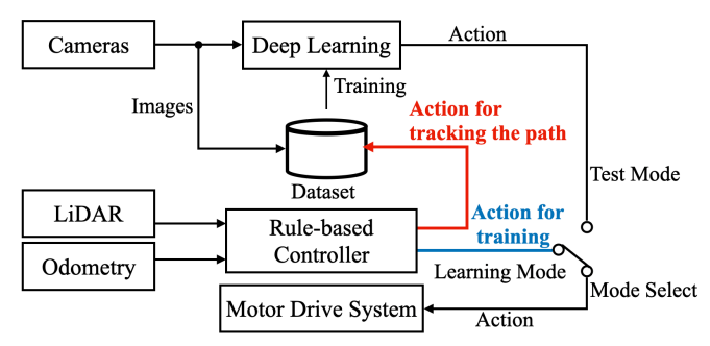
\includegraphics[width=100mm]{images/pdf/okada/method_sys.pdf}
   \caption[Structure of the Okada and others proposed system]{Structure of the Okada and others proposed system(Quoted from\cite{okada2020})}
   \label{fig:okada_sys}
\end{figure}

訓練時には,ROS の navigation パッケージ \cite{ros}を使用して,設定した経路を追従する.
ロボットの並進速度は 0.2 m/sに固定する.
その際,ロボットに取り付けたカメラから取得した RGB 画像とルールベース制御器が出力するヨー方向の角速度をペアにして, 0.2 秒の周期でデータセットに追加する.
収集には 3 台のカメラを使用することで,データの多様性を高めるとともに過学習を防ぐ効果を狙っている.
また,左右のカメラ画像に対するヨー方向の角速度には経路復帰を補助するためのオフセット(\(\pm 0.2\)rad/s)を加える.

\newpage
\figref{fig:okada_net}に岡田らの従来手法における学習器のネットワーク構造を示す.
% 学習器は入力をRGB画像データ,出力をロボットのヨー方向の角速度としている.
ネットワークは,入力層 1,畳み込み層 3,全結合層 2,出力層 1 の全7層で構成される.
データセットからはバッチサイズ 8 で教師データを抽出し, end-to-end 学習を行う.

\begin{figure}[htbp]
    \centering
     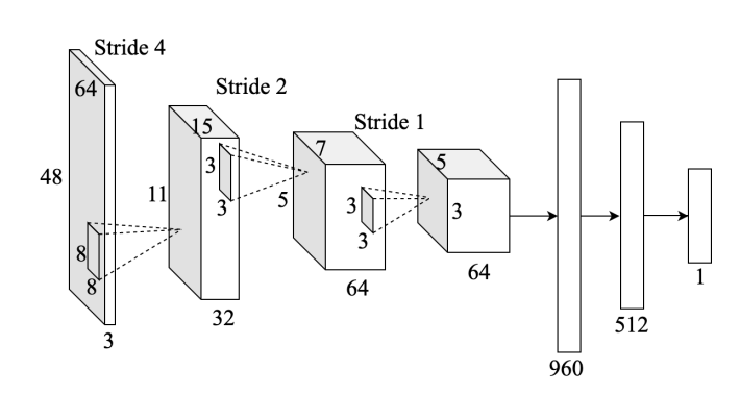
\includegraphics[width=100mm]{images/pdf/okada/network.pdf}
     \caption[Structure of the network Okada and others used]{Structure of the network Okada and others used (Quoted from \cite{okada2020})}
     \label{fig:okada_net}
\end{figure}

学習器の訓練後は,中央のカメラから得た RGB 画像を入力とし,出力されるヨー方向の角速度を用いて経路を追従する.
% この手法は実ロボットを用いて有効性が調査されており,\figref{fig:cource}に示す学習した経路を,画像のみを入力とした学習器の出力で自律移動できることが確認されている.
この手法は実ロボットを用いて有効性が調査されており,学習した経路を画像のみを入力とした学習器の出力で経路追従できることが確認されている.
% \begin{figure}[htbp]
%   \centering
%    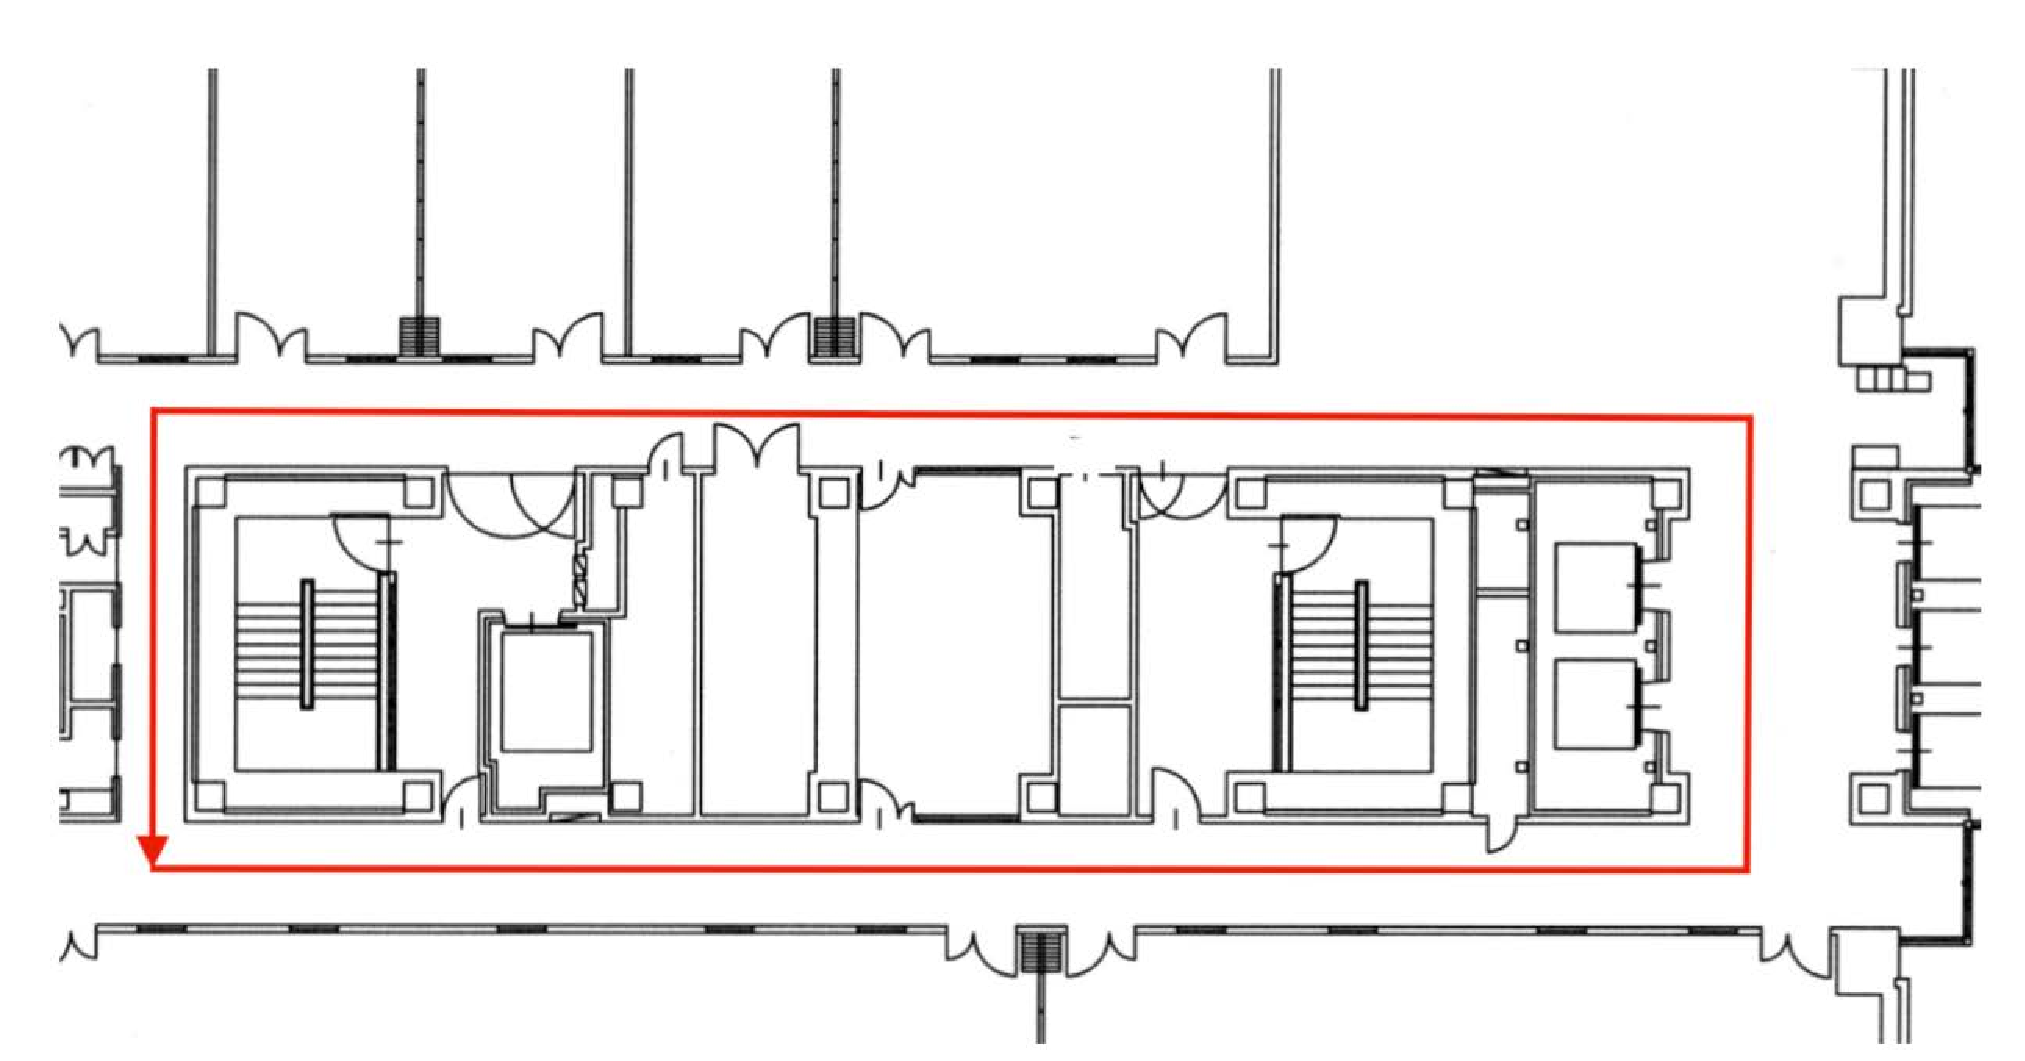
\includegraphics[width=80mm]{images/pdf/okada/cource.pdf}
%    \caption{Target path used in the experiment(Quoted from \cite{okada2020})}
%    \label{fig:cource}
% \end{figure}
